\documentclass[a4paper,11pt]{article}
\usepackage{a4wide,amsmath,ngerman,url,graphicx}
\usepackage[utf8]{inputenc}
\parskip4pt
\parindent0pt

\newcommand{\br}[1]{\left(#1\right)}
\newcommand{\erf}{\mathrm{erf}}
\newcommand{\m}{\cdot}

\title{Analyse der Coronastatistiken. Teil 2} 
\author{Hans-Gert Gräbe, Leipzig}
\date{Version vom 31.05.2020}

\begin{document}
\maketitle

Dieser Text ist eine Fortschreibung des ersten Teils. Die dortigen
Beschreibungen der allgemeinen Rahmenbedingungen werden als bekannt
vorausgesetzt. 

\section{Logistische Funktion}

Generell ist ein Modell auf der Basis einer \emph{Logistischen Funktion}
\begin{gather*}
  u(t)=\frac{K}{1+C\m\exp(-rt)}\tag{L.1}
\end{gather*}
die anerkanntere Form der Modellierung der Ausbreitung einer Infektion, siehe
dazu den entsprechenden Wikipedia-Eintrag. 
\begin{center}
  \includegraphics[width=.8\textwidth]{LC.png}\\[1em] {Logistische Kurve
    $u(t)=\frac{1}{1+12\exp(-2t)}$ (blau)\\ sowie deren erste (rot) und zweite
    (grün) Ableitung}
\end{center}
$K$ steht dabei für die Sättigungsgrenze $\lim_{t\to\infty}{u(t)}$ und $C$ ist
üblicherweise als $C=\frac{K}{u(0)}-1$ angeschrieben, was sich unmittelbar aus
der Umstellung der Formel für $u(0)$ nach $C$ ergibt. Der Wendepunkt dieser
Funktion und damit das Maximum der ersten Ableitung liegt als Nullstelle der
zweiten Ableitung bei $t_0$ mit $u(t_0)=\frac12\,K$. 

Derartige (inhärent transzendente) Funktionen lassen sich aber deutlich
schlechter schätzen als Glockenkurven, die im Teil 1 dieser Reihe betrachtet
wurden und sich durch Logarithmieren auf einfache Weise auf einen polynomialen
Zusammenhang reduzieren lassen.  Siehe hierzu aber die Arbeit von (Engel 2010)
und die Modellierung mit \textsc{GeoGebra} in (Elschenbroich 2020).

In (Engel 2010) wird insbesondere darauf hingewiesen, dass sich mit einer
guten Schätzung von $K$ die anderen beiden Parameter dann doch mit einem
linearen Fitting bestimmen lassen.  Wir transformieren dazu (L.1) in die
Formel 
\begin{gather*}
  l(t)=\frac{K}{1+\exp(-r(t-m))},\tag{L.2}
\end{gather*}
indem $C=\exp(r m)$ ersetzt wird.  Weiter logarithmieren wir (L.2) und
erhalten als neuen Schätzzusammenhang
\begin{gather*}
  \log\br{\frac{K}{l(t)}-1}=-r(t-m)  \tag{L.3}
\end{gather*}
umstellen lässt.  Der Parameter $K$ ist dabei manuell zu schätzen, so dass die
gefittete Kurve möglichst gut auf die Daten passt.  Wir verwenden $K\approx
2A$ aus den Schätzungen der Modellierung im Teil 1.  Die Schätzung für $m$ als
„Höhepunkt“ der Pandemiewelle kann dann mit den Schätzungen im Teil 1
verglichen werden.

Im Skript ist das Ganze in einer Funktion \texttt{lFit(G,K0)} implementiert,
der eine Liste $G$ von Datenpunkten und der Schätzer für $K$ übergeben werden,
wobei in $G$ zusätzlich vorab alle Datenpunkte mit $y_t\le 10$ ausgefiltert
sind.  Dazu wird eine Funktion \texttt{selectData(G,von,bis)} definiert, mit
der aus einer Datenreihe die entsprechenden Daten mit $von<t<bis$ selektiert
werden können.

Wendet man das Verfahren auf die Zahl der positiv getesteten Personen
für die Tage $30\dots 100$ an, so ergeben sich im Wesentlichen die bereits
früher (Stand 10.04.2020 = Tag 101) geschätzten Werte. Allein die Werte für
die Provinz Hebei weichen von den früher berechneten ab.
\begin{center}
  \begin{tabular}{|l|c|c|c|}\hline
    Land & $K$ & $r$ & $m$ \\\hline
    Deutschland & 125\,000 & 0.198 & 91.11\\
    Italien & 145\,000 & 0.207 & 84.47\\
    Österreich & 13\,000 & 0.268 & 85.90 \\
    Spanien & 160\,000 & 0.269 & 88.42 \\
    China (Hebei, alt) & 70\,000 & 0.103 & 45.12\\
    China (Hebei, neu) & 70\,000 & 0.077 & 33.58\\\hline
  \end{tabular}
\end{center}
Die Schätzungen wurden zu einer Zeit ausgeführt, als nur Daten bis zum Tag 100
vorlagen.  Wir sehen an den folgenden beiden Bildern, dass die Schätzungen
wenig dem weiteren Verlauf entsprechen.  
\begin{center}
  \begin{minipage}{.48\textwidth}\centering
    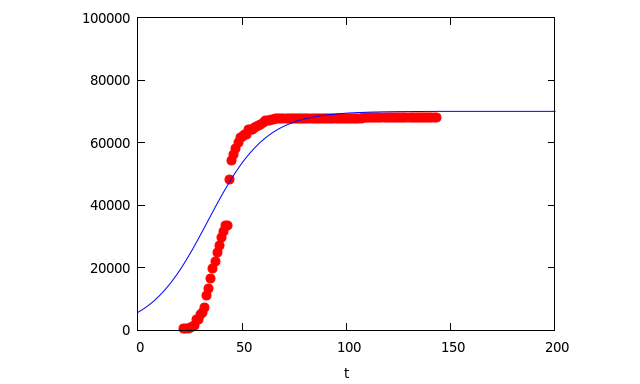
\includegraphics[width=\textwidth]{China-1.png}\\[1em]
                    {Szenario für China (Hebei)}
  \end{minipage}\hfill
  \begin{minipage}{.48\textwidth}\centering
    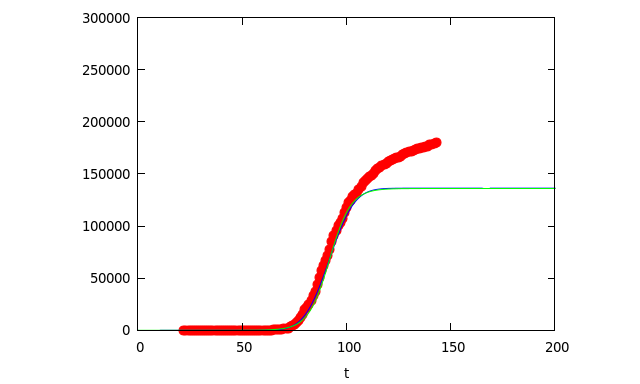
\includegraphics[width=\textwidth]{Germany-1.png}\\[1em]
                    {Szenario für Deutschland}
  \end{minipage}
\end{center}
Mit späteren Daten kann $K$ genauer geschätzt werden. Außerdem zeigen
Experimente, dass Intervalle von etwa $m-25<t<m+25$ besonders gute Schätzungen
liefern. In der folgenden Tabelle sind Schätzungen aus entsprechenden
Zeitreihen der positiv Getesteten für verschiedene Länder gegenübergestellt,
die durch entsprechende Parameteradjustierungen auf Daten bis zum Tag 143
(22. Mai 2020) gewonnen wurden:
\begin{center}
  \begin{tabular}{|l|c|c|c|c|c|}\hline
    Land & $K$ & von & bis & $r$ & $m$ \\\hline
    Deutschland & 200\,000 & 70 & 120 & 0.116 & 100.34\\
    Italien & 250\,000 & 70 & 120 & 0.056 & 103.15\\
    Österreich & 18\,000 & 70 & 120 & 0.116 & 95.30 \\
    Spanien & 270\,000 & 70 & 120 & 0.118 & 100.81 \\
    China (Hebei) & 70\,000 & 22 & 62 & 0.213 & 42.51\\
    Schweden & 50\,000 & 100 & 150 & 0.048 & 128.96\\\hline
  \end{tabular}
  \vskip1em

  \begin{minipage}{.3\textwidth}\centering
    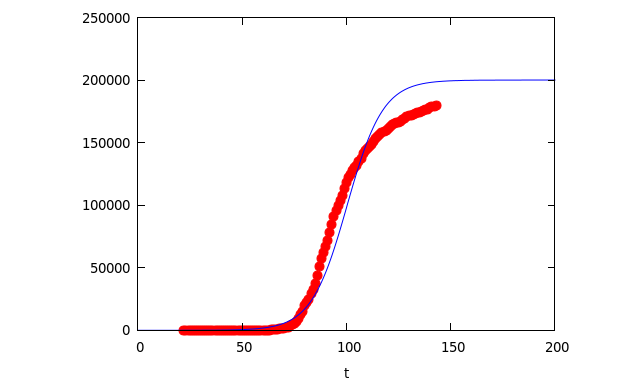
\includegraphics[width=\textwidth]{Germany-2.png}\\[1em] {Deutschland}
  \end{minipage}\hfill
  \begin{minipage}{.3\textwidth}\centering
    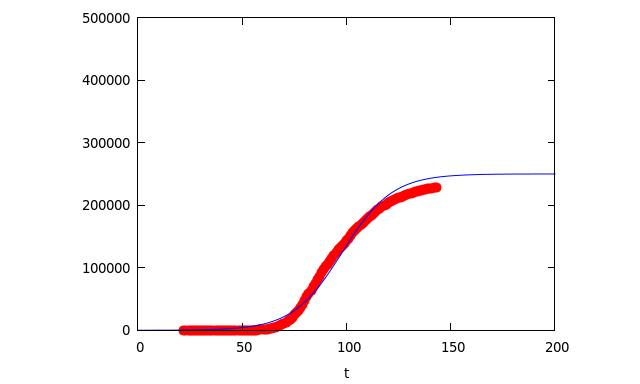
\includegraphics[width=\textwidth]{Italy-2.png}\\[1em] {Italien}
  \end{minipage}\hfill
  \begin{minipage}{.3\textwidth}\centering
    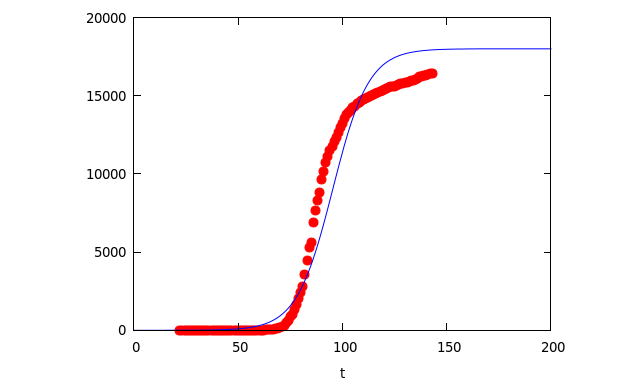
\includegraphics[width=\textwidth]{Austria-2.png}\\[1em] {Österreich}
  \end{minipage}
  
  \begin{minipage}{.3\textwidth}\centering
    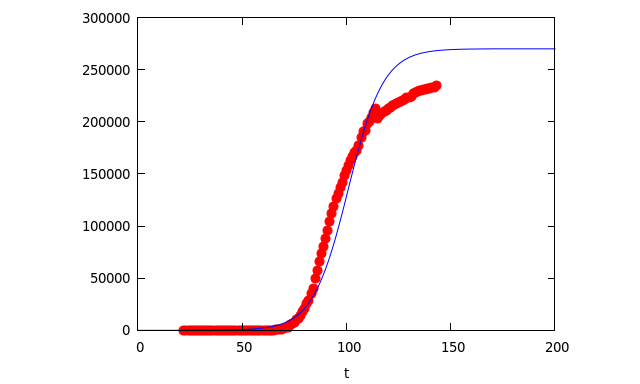
\includegraphics[width=\textwidth]{Spain-2.png}\\[1em] {Spanien}
  \end{minipage}\hfill
  \begin{minipage}{.3\textwidth}\centering
    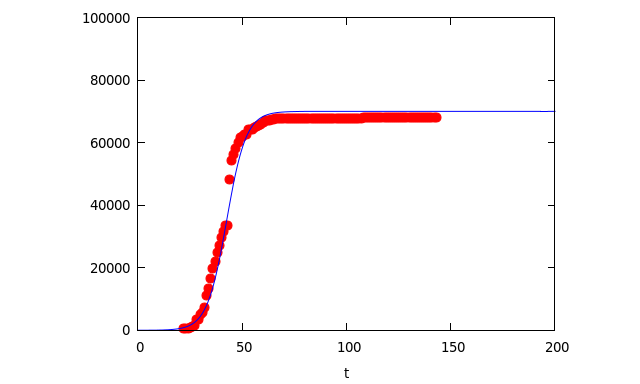
\includegraphics[width=\textwidth]{China-2.png}\\[1em] {China (Hebei)}
  \end{minipage}\hfill
  \begin{minipage}{.3\textwidth}\centering
    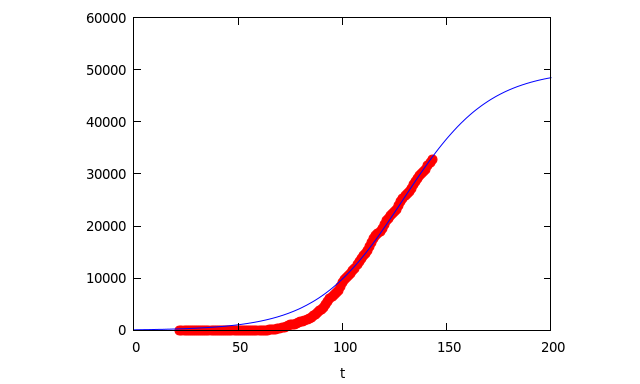
\includegraphics[width=\textwidth]{Sweden-2.png}\\[1em] {Schweden}
  \end{minipage}
\end{center}


\section{Die „Verdoppelungsdebatte“}

Anfang April 2020 kommt eine Diskussion hoch, dass man die rigiden
Beschränkungen erst aufheben könne, wenn „die Verdopplungszeit der Infektionen
größer als 14 Tage“ sei.  Maß kann auch hier nur die Zahl der positiv
Getesteten sein. 

So meldet zum Beispiel der Deutschlandfunk am 04.04.2020\footnote{\raggedright
  \url{https://www.deutschlandfunk.de/covid19-verdopplungszeit-der-coronavirus-infektionen-in.1939.de.html?drn:news_id=1117169}}
\begin{quote}
  Die Verdopplungszeit der Ausbreitung von Coronavirus-Infektionen in
  Deutsch"|land hat sich in den vergangenen Tagen verlangsamt.

  Für ganz Deutschland liegt sie nun bei 11{,}2 Tagen. Die Lage in den
  Bundesländern ist unterschiedlich. In den großen Flächenländern liegt die
  Verdopplungszeit in Nordrhein-Westfalen bei 13{,}1 Tagen, in
  Baden-Württemberg bei 12{,}5 Tagen und in Bayern bei 9{,}7 Tagen. In Berlin
  sind es inzwischen 12{,}8 Tage, in Hamburg 12{,}4. Im Saarland hingegen
  liegt die Verdoppelungszeit bei 5{,}5 Tagen, in Sachsen bei 11{,}0 Tagen.
\end{quote}
Auch wenn dies nicht immer deutlich wird, bezieht sich die Verdopplungszeit
$v_t$ auf die kumulierten Daten und steigt deshalb bereits durch die schiere
Masse der positiv Getesteten.  Ist $y(t)=mt+n$ ein linearer Zusammenhang, so
ergibt sich $v_t=\frac{y(t)}{m}$. Für einen annähernd linearen Zusammenhang
kann man also $v_t=\frac{y(t)}{y'(t)}$ als Schätzung nehmen.  Die Zahl lässt
sich auch aus unseren Daten leicht berechnen: Ist $y_t$ die kumulierte Zahl
der positiv Getesteten am Tag $t$ und $d_t$ die Zahl der (getesteten)
Neuinfektionen, so ist nach $v_t=\frac{y_t}{d_t}$ Tagen eine Verdopplung der
positv Getesteten erreicht, die Zuwachsrate $d_t$ über diesen Zeitraum als
konstant vorausgesetzt.  Beide Datenreihen (Stand 10.04.2020) hatten wir schon
oben extrahiert, so dass wir eine einfache Funktion \texttt{doublePlot(Land)}
schreiben können, um die folgenden Plots zu erzeugen:
\begin{center}  
  \begin{minipage}{.33\textwidth}\centering
    \includegraphics[width=\textwidth]{Italy-DP.png}\\[1em] {Italien}
  \end{minipage}\hfill
  \begin{minipage}{.33\textwidth}\centering
    \includegraphics[width=\textwidth]{Germany-DP.png}\\[1em] {Deutschland}
  \end{minipage}\hfill
  \begin{minipage}{.33\textwidth}\centering
    \includegraphics[width=\textwidth]{Austria-DP.png}\\[1em] {Österreich}
  \end{minipage}
\end{center}


\section{Literatur}

\begin{itemize}
\item Hans-Jürgen Elschenbroich. Corona: Mathematik \& Modellbildung.\\
  \url{https://www.geogebra.org/m/cfammtpe}.  2020.
\item Joachim Engel. Parameterschätzen in logistischen Wachstumsmodellen.
  Stochastik in der Schule 30 (2010) 1, S. 13–18.
\end{itemize}

\end{document}
